\documentclass{article}
\usepackage{tikz}
\usepackage[american]{circuitikz}

\usetikzlibrary{arrows,decorations.markings}

\title{Computer Organization and Architecture}
\author{Conrad A. Mearns}

\begin{document}

\maketitle

\section{Turing Machines}
\begin{enumerate}
  \item {Turing's Thesis: Every computation can be represented with a Turing Machine.}
  \item {Turing Machine: A mathematical model of a device that can preform any computation.}
  \item {Universal Turing Machine: A machine to implement any and all Turing Machines.}
\end{enumerate}

Beyond models, real world constraints include time, financial cost, power, security, thermal dissapation, space, etc.\\

\section{Bits, Data Types, and Operators}
The electro-magnetic field is not digital, yet all of modern computing is represented digitally. To compromise, 0 is a representation of the absence of voltage and 1 is a representation of the presence of voltage.

\centering
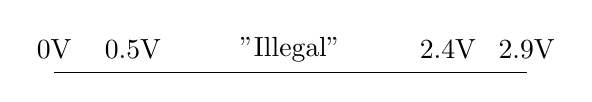
\begin{tikzpicture}
  \node (a) at (0,1) {0V};
  \node (b) at (1,1) {0.5V};
  \node (c) at (5,1) {2.4V};
  \node (d) at (6,1) {2.9V};
  \node (b) at (3,1) {"Illegal"};
  \draw (0,.7) -- (6,.7);
\end{tikzpicture}
\raggedright

\section{Signed Binary Arithmetic}
Binary, without the addition of extra mathematical symbols, can only represent positive whole integers. Signed numbers like $-5$ require a formal system of representation in order to be used. A binary number can represent $2^n$ values for $n$ bits. The objective of signed numbers is to partition half of those values for negative number representation ($-2^{n-1}-1 \to -1$) and the other half to positive numbers ($1 \to 2^{n-1}$) while leaving zero and potentially one other number available.

\begin{enumerate}
  \item {
  Sign-Magnitude\\
  The most significant bit is 0 for positive values and 1 for negative values.\\
  $00101 = 5$ and $10101 = -5$
  }
  \item {
  One's Complement\\
  All bits are inversed to represent negative numbers. Like Sign-Magnitude, the most significant bit will tell you whether a number is positive or negative.\\
  $00101 = 5$ and $11010 = -5$
  }
  \item {
  Two's Complement (currently in use)\\
  For each positive number $A$, it's negative number ($B$) satisfies the equation $A + B = 0$ when the final carried bit is dropped. To get this number, take the One's Complement of $A$ and add 1.
  $00101 = 5$ and the One's Complement is $11010$. So the Two's Complement is $11011$. As proof, $00101 + 11011 = 100000$ but the last carried one is dropped, leaving $00000$.
  }
\end{enumerate}

\section{Arithmetic and Logical Operations}
Arithmetic operations
\begin{enumerate}
  \item {Addition\\Just addition, regardless if signed or not. Ignore the final carry-out.}
  \item {Subtraction\\First negate the second operand ($5 \to -5 for example$), then use addition.}
  \item {Sign Extension\\To add numbers, they must have the same number of bits. This is because of signed numbers, and storage.}
\end{enumerate}

Overflow occurs when
\begin{enumerate}
  \item Signs of the operands are the same
  \item The sign of the sum is different
\end{enumerate}
The issue can be tested for by examining the most significant bit's sign between the operands and the result.

Logical operations
\begin{enumerate}
  \item {AND\\The result is true if and only if both operands are true.\\Useful for clearing bits, a mask of 1's signify keep.}
  \item {OR\\The result is true if either operand is true.\\Useful for setting bits. 1's in the second operand copy to the result.}
  \item {NOT\\The result is true if and only if the operand is false.}
\end{enumerate}
\noindent
Each operation is executed on each bit individually.

\section{Fractions, Floating, and Fixed-Point Values}
A "binary" point is abstractly added to the value. To the left of the point, each bit is worth is $2^{-n}$ where n is the place left of the point. For example, $101.11$.

For large numbers, we use scientific notation. $Sign * (Fraction * 2^{Exponent})$
IEEE 754 Floating Point Standard for 32-bits signifies 1 bit for sign, 8 bits for the exponenant, and 23 bits for the fraction.
$1-01111110-10000000000000000000000 = -1.5*2^{???}$

\section{Other Date Types}
\begin{enumerate}
  \item Single characters use ASCII to map 128 characters to 7-bit code.
  \item Text strings are sequences of characters often with a NULL to terminate. No hardware support.
  \item Images are arrays of images. Often has hardware support.
  \item Sound is a sequence of fixed-point numbers.
  \item Other data types my be defined abstractly by us and interpreted as needed.
\end{enumerate}

\section{Transistors}
Each transistor is a digital switch. When combined in different circuits, transitor combinations can emulate certain logical operations such as AND, OR, and NOT. These can then be combined to create adders, multiplexers, decoders, and other farther complex structures.\\
Gordon Moore, an early founder of Intel, hypothesized that transistor count would double every two years. This is now known as Moore's Law.\\
Transitors have 3 wells. A well is a homogeneous material that is either more or less positive than negative. A negative well is denoted $n$ and a positive well is denoted $p$. The gate in a transitor creates a field to allow or dissallow charge to migrate across wells.

n-Type Transistor (npn)\\
Two $n$ wells inside a large $p$ substrate.
\begin{itemize}
  \item When gate is tied to GND, the switch is open.\\
    No current flows from the source to the drain.\\
    '0 state'
  \item When gate is tied to voltage the switch is closed.\\
    Current flows from the source to the drain.\\
    '1 state'
\end{itemize}

p-Type Transistor (pnp)\\
Two $p$ wells inside a large $n$ substrate.
\begin{itemize}
  \item When gate is tied to GND, the switch is closed.\\
    Current flows from the source to the drain.\\
    '1 state'
  \item When gate is tied to voltage the switch is open.\\
    No current flows from the source to the drain.\\
    '0 state'
\end{itemize}

\section{Complementary Metal Oxide Semiconductor Circuits(CMOS)}
\begin{itemize}
  \item NOT Gate (Inverter)
  \item NOR Gate (NOT OR, Serial on top, Parallel on bottom)
  \item OR Gate (NOR + NOT)
  \item NAND Gate (NOT AND, Parallel on top, Series on bottom)
  \item AND Gate (NAND + NOT)
\end{itemize}

\section{Simplified Gates}
\begin{itemize}
  \item {
  NOT Gate\\
  \begin{circuitikz}
    \draw (0,0) node[not port]{} (2,0);
  \end{circuitikz}
  }
  \item {
  OR Gate\\
  \begin{circuitikz}
    \draw (0,0) node[or port]{} (2,0);
  \end{circuitikz}
  }
  \item {
  NOR Gate\\
  \begin{circuitikz}
    \draw (0,0) node[nor port]{} (2,0);
  \end{circuitikz}
  }
  \item {
  AND Gate\\
  \begin{circuitikz}
    \draw (0,0) node[and port]{} (2,0);
  \end{circuitikz}
  }
  \item {
  NAND Gate\\
  \begin{circuitikz}
    \draw (0,0) node[nand port]{} (2,0);
  \end{circuitikz}
  }
\end{itemize}

\section{Other Circuits}
\begin{itemize}
  \item 2-Bit Decoder\\
    Uses 4 AND Gates with different inverter configurations on each. It maps 2 inputs to 4 outputs.
  \item Multiplexer\\
  Uses 4 inputs and interprets to 1 output. A selector input of two wires will change the output from 4 AND Gates.
  \item Full Adder\\
    Capable of adding two bits with carry-in. Produces a one-bit sum with carry-out
\end{itemize}

\section{Logical Completeness}
Can complete any truth table with just AND, OR, NOT. First, mark every output row that has a truth value of true. Draw an OR gate at the bottom to accept all true outputs. Connect AND Gates to the OR Gate and have every input connect to each AND gate. For each AND Gate, configure the inputs with invertes so that each AND Gate emulates a truth table row.

\section{Combinational vs Sequential Circuits}
Combinational Circuit\\
always produces the same output for a given set of inputs\\
Sequential Circuit\\
Stores information\\
Output depends on stored information (state) plus input

\section{R-S Latch}
R is used to 'Reset' or clear the element - set it to zero.\\
S is used to 'set' the element - set it to one.\\
If both R and S are one, the output could be either one or zero. To assert one of the inputs, use Active Low Logic.\\

\section{Gated D Latch}
Based upon R-S Latch and has 2 inputs. D (for data) and WE (write enabled). Two AND gates feed into the R and S inputs of an R-S latch, and input is only sent to the R-S latch when WE is asserted.\\
WE = 1 $\to$ latch is set to the value of D. S = NOT(D), R = D\\
WE = 0 $\to$ latch holds previous value. S = R = 1\\

\section{Register}
Side by side Gated D latches that share a single WE line, but has seperate data lines.\\
A register holds a n-bit value, controlled by a common WE.\\

\section{Memory}
Address is taken as multple inputs, that input passes to an address decoder which uses AND gates to specify what memory location can be written to, when WE is asserted.\\
Not the most expensive, and more transistors are needed in greater desnity.\\
Address decoder\\
Word Select Line\\
Word Write Enable

\section{Representing Multi-bit Numbers}
Number bits from right to left for convention. Use brackets to denote range.\\
D[l:r] denotes bit l to bit r from left to right in register D\\
May also see "A<14:9>"\\

\section{State Machine}
Finite State Machine with Datapath (FSMD)\\
Controller / Data Path\\
Another type of combinational logic with storage. It "Remembers" states and changes it's output(s) are based on inputs and the state machine's current state. This type of circuit is the heart of the controller in a CPU.\\

Combinational vs Sequential: Combinational types depend only on the values. Sequential types sctrictly depend on the order of values inputted.

The state of a system is a snapshot of all the relevant elements of the system at the moment the snapshot is taken.

State diagrams are directed graphs that show how actions change states.

\begin{enumerate}
  \item A finite number of states
  \item A finite number of external inputs
  \item A finite number of external outputs
  \item An explicit specification of all state transitions
  \item An explicit specification of what determines each external value
\end{enumerate}

Clock cycles are used in digital circuits to trigger state transitions. A single cycle is when the value changes between '1' and '0' fully. Transitions can be triggered with edge triggered logic, or level triggered logic.

Storage for state machines can be accomplished using a Master-Slave flipflop.

\section{From Logic to Datapath}
The datapath of a computer is all the logic used to process information.
\begin{itemize}
  \item Combinational Logic\\
  Decoders -- convert instructions into control signals\\
  Multiplexers -- select inputs and outputs\\
  ALU (Arithmetic and Logic Unit) -- operations on data\\
  \item Sequential Logic\\
  State machine -- coordinate control signals and data movement\\
  Registers and latches -- storage elements\\
\end{itemize}

\section{von Neumann Machine / Model}
Basic structure of machine that is the most common, even today.\\
a memory, containing instructions and data\\
a processing unit, for preforming arithmetic and logical operations\\
a control unit for interpreting instructions\\

\section{Harvard Model}
Refinement of von Neumann Model.\\
seperate memory for programs and data\\

Both models are sequential and synchronous. Programs are both interpreted by a control unit.

\begin{itemize}
  \item IR - Instruction Register
  \item PC - Program Counter
  \item ALU - Arithmetic and Logical Unit
  \item MAR - Memory Address Register
  \item MDR - Memory Data Register
  \item PMEM - Program Memory (Harvard Model, effectively Read-Only)
  \item DMEM - Data Memory (Harvard Model)
\end{itemize}

\section{Memory}
$2^k * m$ array of stored bits.\\
Address - unique k-bit identifier of location\\
Contents - m-bit value stored in location\\

Basic Operations:\\
LOAD - Read a value from a memory location\\
STORE - Write a value to a memory location\\

\section{Interface to Memory}
To LOAD a location (A)
\begin{itemize}
  \item Write the address (A) into the MAR
  \item Send a 'read' signal to the memory
  \item Read the data stored in MDR
\end{itemize}

To WRITE a value (X) to a location (A)
\begin{itemize}
  \item Write data (X) to the MDR
  \item Write the address (A) to the MAR
  \item send a 'write' signal to the memory
\end{itemize}

\section{Processing Unit}
Functional Units - add, multiply, square root\\
Registers - Small temp storage, operands and results of functional units\\
Data Word Size - number of bits normally processed by ALU in one instruction. Also the width of registers\\

\section{Input and Output}
\begin{itemize}
  \item Devices for getting data into and out of computer memory
  \item Each device has its own interface, usually a set of registers like the memory's MAR and MDR
  \item Some devices provide both input and output (disk, networking)
  \item Programs that control access to a device is a driver
\end{itemize}

\section{Control Unit}
\begin{itemize}
  \item Instruction Register - IR - contains the current instruction
  \item Program Counter - PC - contains the address of the next instruction to be executed
  \item Control unit reads an instruction from memory. interprets the instruction, generating signals tha tell the other components what to do
\end{itemize}

\section{Instruction Processing - PNAMBC}
PNAMBC $\to$ Pay No Attention to the Man Behind the Curtain
\begin{itemize}
  \item Fetch instruction from memory
  \item Decode instruction
  \item Evaluate address
  \item Fetch operands from memory
  \item Execute operation
  \item Store result
\end{itemize}
Instructions are the fundemental unit of work. An instruction specifies opcode (what operation needs to be preformed) and operands (data/locations to be used in the operation). They are stored just like data, as a fixed length sequence of bits. The Control Unit interperats the instruction and generates a sequence of signals to carry out the action.

A computer's instructions and their formats is known as it's Instruction Set Architecture (ISA)

\section{Types of Instructions}
\begin{itemize}
  \item Computational instructions (ADD, AND, etc)
  \item Data movement instructions (LD, ST, etc)
  \item Control instructions (JMP, BRxx, etc)
\end{itemize}

\subsection{AVR add instruction}
Instruction format: 000011rdddddrrrr\\
For this ISA, 000011 is the opcode for addition, and d is the 'destination register' and r is the 'source register'. The r and d is staggered for legacy reasons.

Syntax: add Rd, Rr\\
Example: "add r1, r3 ; add r3 to r1… bits are 0000110000010011"\\

\subsection{AVR rjump instruction (Relative Jump)}
Instruction format: 1100kkkkkkkkkkkk\\

Syntax: rjump k $-2K \leq k < 2K$\\
Operation: PC = PC + k (after PC is already incremented) where $-2K \leq k \leq 2K$\\
Example: "rjmp DoIt ; jmp to label DoIt… bits are 1100000011111111"\\

\section{Instruction Processing}
\begin{itemize}
  \item {FETCH:
    \begin{itemize}
      \item Load next instruction from the address stored at the program counter (PC) and place into the instruction register (IR)\\
      Copy contents of PC to PMAR (Program Memory Address Register)\\
      Send "read" to memory\\
      Copy PMDR (Program Memory Data Register) contents to IR
      \item Increment the PC so that it points to the next instruction
    \end{itemize}
  }
  \item {DECODE:
    \begin{itemize}
      \item Identify the opcode\\
        For the AVR ADD instrution, this is bits [15:10]
      \item Depending on the opcode, identify the other operands from the remaining bits
    \end{itemize}
  }
  \item {EVALUATE ADDRESS:
    \begin{itemize}
      \item
    \end{itemize}
  }
\end{itemize}

\section{Assembly Language}
Nothing but human readable machine code. Assembly gives a way to easily convert between symbols and machine code.\\
An assembler is a program that makes such a conversion. Assemblers are very specific to ISA. Because of this, there is a very close relationship between symbols and instruction sets. This means opcodes are mnemonics specific to an ISA. Using assembly we can label locations in memory to prevent hassles with program location.

Some instructions can only be preformed on specific registers.

\subsection{Syntax}
LABEL OPCODE OPERANDS ; COMMENTS (where the label and comment are optional)
\begin{itemize}
  \item Comments: begin with a semi-colon\\
  ";This is a comment"
  \item Labels: not a instruction, but a tag within the code that defines a location. In AVR, labels end with a colon\\
  "mylabel:"
  \item Assembler Directive: specifies the origin of the next instruction within memory\\
  ".org 0x100" - this means the next instruction will be at location 0x100
  \item Opcode: can be different per instruction. Generally organized to have a text mnemonic followed by comma sperated values in the form of labels, registers, and numbers.\\
  "ldi r16, 6" - Load the value '6' into register 16
  \item Operands: registers, numbers, labels.\\
  Registers have the format r1, r13, fXX.\\
  Numbers can be decimal X or hex 0xX.\\
  Labels are just text, in the format XXXXX
  \item Directives: pseudo-operations used only by the assembler. Start with a '.'\\
  .ORG [address] - Starting address of next instruction in PMEM\\
  .BYTE [expressions] - Place bytes from expressions in code\\
  .SET [symbol, expression] - Set the value of a symbol to an expression\\
  .FILL [repeat, size, value] - allocate one word, init with a value\\
  .SECTION [section name] - Place following code into the section name's location
\end{itemize}

\section{Register Transfer Language (RTL)}
FETCH\\
$PMAR \Leftarrow PC$\\
$Assert READ of PMEM$\\
$PMDR \Leftarrow PMEM[PMAR]$\\
$IR \Leftarrow PMDR$\\
$PC \Leftarrow PC + 1$

\section{Assembly Process}
Convert's assembly files (.asm) to executables (.hex) for the AVR.

First Pass
\begin{itemize}
  \item Scan assembly file
  \item find all labels and calculate corresponding addresses (symbol table)
\end{itemize}

Second Pass
\begin{itemize}
  \item Convert instructions to machine code using information from the symbol table
\end{itemize}

\subsection{Constructing a Symbol Table}
\begin{enumerate}
  \item Initialize the location counter (LC) which keeps track of the address of the current instruction
  \item For each non-empty line in the program:
  \begin{enumerate}
    \item If the line contains a label, add label and LC to symbol table
    \item Increment LC (If .FILL or .BYTE is used, increment LC by the number of words allocated)
  \end{enumerate}
  \item Stop construction when end of file is reached.
\end{enumerate}

\subsection{Second Pass}
\begin{itemize}
  \item For each executable assembly statement, generate the corresponding machine language instruction
  \item Potential problems:
  \begin{itemize}
    \item Improper number/type of arguements
    \item Immediate arguement too large
  \end{itemize}
\end{itemize}



\end{document}
